% empty template for ARM entry. By Dirk Doornenbal. V1.2 18 april 2006
% Internals entry V1.0 ?? april 2006
\nomenclature{LHS}{Left Hand Side}%
\nomenclature{RHS}{Right Hand Side}%
\nomenclature{EBNF}{Extended Backus-Naur Form}%
\nomenclature{OO}{Object Oriented}%
\chapter{Internals}%\label{insert_label}
Internals are the object instances that are instantiated for each instance of a
filter module. Because of this, internals can be used in situations where
each instance of a filter module must have its own instance of an object, for example
to hold a state or for inheritance by delegation.

\section*{Syntax}
The internal declaration has two parts, which are separated with a colon. The
left hand side contains the identifiers of the internals and the right hand
side the type of those identifiers. 
The formal syntax is defined in \autoref{lst::ARM:int:syntax}.

The types are defined by fully qualified names.
You can refer to an internal in the conditions field,
the filter parameters, and the Target.
Internals can only be objects, primitive types are not allowed.
\begin{lstlisting}[caption = {Internals syntax}, label = lst::ARM:int:syntax,
style = listing, language = ebnf, float = tpb]
FilterModule ::= `filtermodule' FilterModuleName 
                  [FilterModuleParameters] `{'
                  [Internals] [Externals] [Conditions]
                  [InputFilters] [OutputFilters] `}'
Internals ::= `internals' (Identifier-LIST `:' Type `;')*
\end{lstlisting}

\section*{Semantics}
When the filter module gets instantiated, then 
all its internals get instantiated using the constructor with no parameters,
this is often the default constructor.
\autoref{lst::ARM:int:example2} shows the binding of a filter module isActive
to classes A and B. What this code does at run time is shown in \autoref{fig::arm::int:initialisation},
every instance of A and B gets its own instance of the filter module isActive
and each instance of the filter module gets its own instance of the internal \lstinline!state!.

The effect is that every instance of an object gets its own instance of the filter module and thus
indirect the internal, making it suitable for storing states independently and for inheritance by
delegation. With the proper filter construction, like \lstinline!d : Dispatch = { <internal.*> internal.*}!, 
it is possible to extend the signature of a superimposed object with the signature of the internal.
This means that you do not need to access the internal from outside the filter module, because you can directly
use the object on which is superimposed.

\begin{lstlisting}[caption = {Example 2, a filter module to hold a state}, label = lst::ARM:int:example2,
style=listing, language=ComposeStar, float = tpb]
filtermodule isActive{
  internals
    state : State;
  conditions
    notActive : state.notActive();
  inputfilters
    d : Dispatch ={<state.*> state.*};
    e : Error (state) = {notActive => [*.*]}
}
superimposition{
  selectors
    sel = {C | isClassWithNameInList(C,[`A', `B'])};
  filtermodules
    sel <- isActive;
}
\end{lstlisting}

\begin{figure}[tpb]
	\centering
	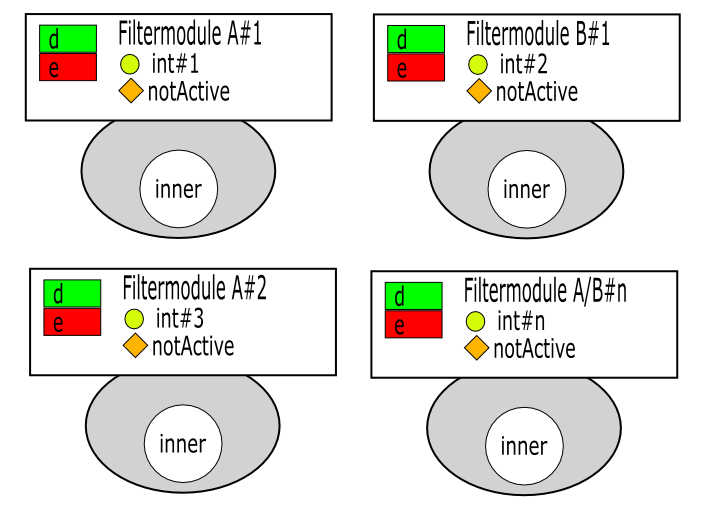
\includegraphics[style=thirdheight]{images/ARM-internalInitialization}
	\caption{Instances of \autoref{lst::ARM:int:example2}}
	\label{fig::arm::int:initialisation}
\end{figure}

\section*{Examples}
In the Pacman example (\autoref{lst::ARM:int:example1}), the strategies
are internals; this gives that they are instantiated for each 
filter module. An internal is declared with a fully qualified name
of a class.

\begin{lstlisting}[caption = {Example 1, a piece of Pacman}, label = lst::ARM:int:example1,
style=listing, language =ComposeStar, float = tpb]
filtermodule dynamicstrategy{
  internals
    stalk_strategy : pacman.Strategies.StalkerStrategy;
    flee_strategy : pacman.Strategies.FleeStrategy;   
  conditions
    ...
\end{lstlisting}

\section*{Legality Rules}
\begin{itemize}[noitemsep]
\item The identifier of an internal must be unique for the filter module where it is declared in;
\item The type must be a fully qualified name of a class and this class must exist;
\item In order to be instantiated, the class for the internal must have a constructor without parameters;
\item When an internal is declared but not used you get a warning from the compiler.
\end{itemize}

\faq{
\para{FAQ}
\question {What is the use of declaring multiple instances of one type? Is it not possible
to rewrite the class of the type, so that you only need to declare one internal?}
\answer {This depends on the situation, whereas for holding a state you can also write
another class that takes care of the complete state, however for constructions
where you delegate to a tree-like structure,
like \lstinline!left, right : Node;!, you do not want to combine the internals into one class.}

\question {Is it possible to access an internal of another filter module?}
\answer {It is not possible, on conceptual and implementation level, to
access an internal with a filter module element reference.}

\question {I want to declare an internal with a type that is in a library, but the class does not have a default constructor.
How can I solve this?}
\answer{The best way to solve this is by extending the class you want to use with a default constructor
that sets the needed default values. If that is not possible because the class has been made final,
then you can write a static method which calls a constructor with arguments and returns the result,
this static method can be used in the declaration of an external\footnote{\nb: Only use this
construction if you are stuck in such particular situation, see also the commentary.}.}
 
\para{Hints}
The instantiation of an internal happens with a constructor with no parameters. In most
object-oriented languages this is the default constructor, which is used when the user
does not create a constructor. Sometimes people forget to create a constructor
without parameters, when there is already a constructor with parameters, which
results in an error.
}

\comments{
\para{The use of Arguments in Constructors Calls}
The internal initialization is done with a constructor without arguments; this is a result of the requirement to be language independent. 
The internal declaration \lstinline!internal: Person = Person(``Albert'', 24, true);! is considered as language dependent and therefore only constructors without arguments are used. 
We will not re-discuss the point of allowing primitive values in the internal declaration, because is has been discussed in \autoref{chapter:filtermodule}.
However, with the introduction of the filter module parameters it is possible to use objects, which are passed through the filter module parameters, in the declaration of the internals.
This feature is not added to the syntax yet, because it relies on the full implementation of the filter module parameters. 
When this is realized then the syntax can change to the one given in \autoref{lst::ARM:int:syntax2}.
\\\\
\begin{lstlisting}[caption = {Proposed internal syntax}, label = lst::ARM:int:syntax2,
style = listing, language = ebnf]
Internal ::= Identifier {',' Identifier} ':' Type 
              [`=' Fqn `(' FilterModuleParameters `)']
\end{lstlisting}
Because we already use default constructors, we already have the mapping from the language independent declaration to language specific constructor calls, thus we do not have to work them out for adding arguments in a constructor.

\para{Visibility of Internals}
As mentioned in the semantics, it is possible to extend the signature of the class on which is superimposed with the signature of the internal. 
What is not mentioned in the text, is whether the internal is public or private value, and even more important can we directly access the internal?
To start with the public or private matter, addressing the filter module directly from outside the filter module is not correct programming for Compose*, because it breaks with the filter interface. 
So whether it is public or private, you should not access it anyway.

\para{Internals as Externals}
As mentioned earlier in \autoref{chapter:filtermodule} it is good to keep a difference between internals and externals.
It is however, possible to write all internals as externals, if you write a static method \lstinline! static public getnewPerson() \{ return new Person() \} ! and you use that in an external declaration, \lstinline!externals person : Person = person.getNewPerson()!, then you get the same result as when you would create an internal with \lstinline !internals person : Person!.
The construction showed here is not what we want, because we break the decoupling of the main code and the concerns, the class Person, which is in the main code, does have a method which is solely written for a concern.
The only correct use for this construction is when you want to use an internal of a class out of a library, and this class does not have a default constructor and the class is declared as final\footnote{It is actually your only option when you are stuck with such a library.}. 
It is for the best to avoid this kind of constructions; however it is good to know that there are workarounds for this kind of situations.

\para{Visibility of Internals}
As mentioned in the semantics, it is possible to extend the signature of the
class on which is superimposed with the signature of the internal. What is not mentioned in the text, is whether the internal is
public or private value, and even more important can we directly access the internal?
To start with the public or private matter, addressing the filter module directly from outside the filter module is not
correct programming for Compose*, because it breaks with the filter interface. So whether it is public or private, you should not access it anyway.

\para{Internals as Externals}
As mentioned earlier in \autoref{chapter:filtermodule} it is good to keep a difference between internals
and externals.
It is however, possible
to write all internals as externals, if you write a static method
\lstinline! static public getnewPerson() \{ return new Person() \} ! and you use that in
an external declaration, \lstinline!externals person : Person = person.getNewPerson()!,
then you get the same result as
when you would create an internal with \lstinline !internals person : Person!.
The construction showed here is not what we want, because we break the decoupling of
the main code and the concerns, the class Person, which is in the main code, does have a method which is
solely written for a concern. The only correct use for this construction is when you
want to use an internal of a class out of a library, and this class does not have a default constructor
and the class is declared as final\footnote{It is actually your only option when you
are stuck with such a library.}. It is for the best to avoid this kind of constructions;
however it is good to know that there are workarounds for this kind of situations.
}

\dotnetcomment{
If you really want to access an internal then there are two options,
first you can access the filter information from the repository, which has at runtime the reference
to the internal you want. %\footnote{As you might guessed this is actually a hack.}.
Second, it is possible to write a filter that returns the internal and with the
extension of the signature of the superimposed object you can get a \emph{get-method}
for the internal, this construction is demonstrated in \autoref{lst::ARM:fmp:commentdotnet1}. 
The second option
is preferable above the first one, because it is more clear of what you do, only in
certain cases where you cannot extend the signature you are stuck with the first option.
If you really want to access an internal then there are two options, first you can access the filter information from the repository, which has at runtime the reference to the internal you want. 
%\footnote{As you might guessed this is actually a hack.}.
Second, it is possible to write a filter that returns the internal and with the extension of the signature of the superimposed object you can get a \emph{get-method} for the internal, this construction is demonstrated in \autoref{lst::ARM:fmp:commentdotnet1}. 
The second option is preferable above the first one, because it is more clear of what you do, only in certain cases where you cannot extend the signature you are stuck with the first option.

\begin{lstlisting}[caption = {How to get hold of an internal}, label = lst::ARM:fmp:commentdotnet1,
style = listing, language=ComposeStar, float = tpb]
filtermodule returnInternal{
  internals
    state : State;
  inputfilters
    d : Dispatch = {[*.getState] s.getSelf}
}
\end{lstlisting}
}

%\ccomment{To be specified\\\\\\\\\\}

%\pending{}

%\furtherreading{}

